We decided to base our application on~\nameref{subsec:git-time-metric} and have the time tracking data stored in Git Notes
for every repo so that it can be tightly tied to code.
This gives us an opportunity to have a more complete overview of when and on what issue/branch the time was spent.
It also gives access to features such as Git diff that can be used for measuring writing speed.
Furthermore, it lifts a job from our shoulders by handling complex cases such as rebase and merge for us.

The downside is that Git notes take up some space on the client machine(s) and Git server.
They can also be externally edited, and they might cause issues with Git usage if the developer does not follow best practices.
Nonetheless, we decided to go this way as the space used by Git notes is fractional compared to file sizes, and our app is a tool for the developer,
so we don't see any urgent need to protect it from him.

Later it was brought out in Gitlab time tracking issue discussion, that they consider storing time data in Git notes
to be a very clean approach compared to storing it in commit messages.
However, they have not yet decided to implement it themselves as it requires major changes in their current business logic.
\cite{gitlab-time-issue}

Partly enforced by the usage of Git, the general design is shown in Figure
\ref{fig:project-archidecture}.

\begin{figure}[h]
    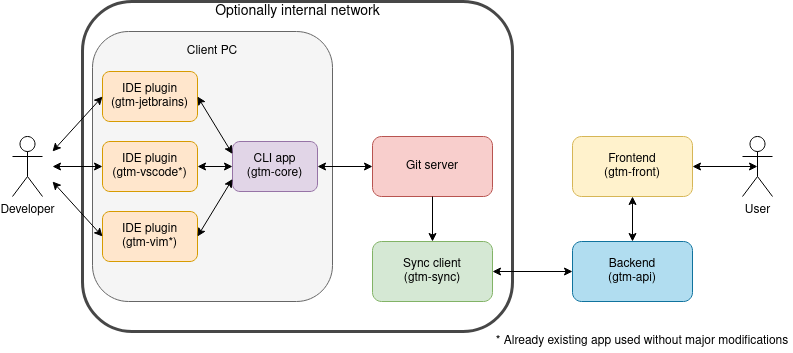
\includegraphics[width=\textwidth]{figures/project_archidecture}
    \caption{Application general design}
    \label{fig:project-archidecture}
\end{figure}

The general time-tracking application can be divided into three different kinds of smaller applications:
\begin{enumerate}
    \item \textbf{Applications that are responsible for data collecting.} These applications are CLI app and IDE plugins and are installed on the developers machine.
    \item \textbf{Applications that are responsible for syncing data.} This role is filled by a Sync client.
    These applications can be installed onto companies/universities servers where they can access Git's internal network if needed.
    \item \textbf{Applications that are responsible for analysing and displaying data.} These are Frontend and Backend apps that are installed on any server.
\end{enumerate}

The reasoning behind this architecture is security and scalability.
For every backend there can be multiple Sync clients all installed on different machines and with different Git access rights.
For every Sync client, there can be multiple client apps all logging time independent of one another.
And in the end, there can be multiple IDE plugins interacting with CLI app.

For security, it is very important to ensure, that no sensitive information is leaked.
To deal with this issue many companies have their Git available only in an internal network.
Not to raise any more security concerns we decided to follow the same principle and not export any Git code outside an internal network.
That is the reason, why Sync client is needed as it has access to the internal network, but only uploads time-tracking related information to our backend.
Therefore, actual code never leaves the internal network.

All the applications that are installed on either client machine or client's server are open source so that the client can easily verify,
they only do what they are meant to do and perform no malicious activities.

To properly manage numerous apps in different programming languages we decided to have each app source code in a separate Git repository.
This reduces the number of merge conflicts and also makes building CI/CD easier.


\section{Client CLI app}\label{sec:cli-app}
%TODO(Tavo): We should somewhere state what are gtm-core, gtm-api, gtm-*
This is the main app on the client machine.
The app is responsible for storing events sent by an editor to files and then later also combining the stored information into Git Note.
You can also see all main stats, such as time spent on a commit via CLI app.

The app is based on open source time tracking app \href{https://github.com/git-time-metric/gtm}{Git-Time-Metric} written in Go and licensed under MIT licence.
We decided to base our app on Git-Time-Metric solution because their app was working the way we wanted to, it had plenty of users meaning plenty of testing done,
and the Git-Time-Metric app had a good code style.

Gtm-core folder structure is displayed in Table
\ref{tab:gtm-core-folder-structure}.

\begin{table}[h]
    \centering
    \begin{tabular}{ | p{3cm} | p{10cm} |}
        \hline
        \textbf{Folder} & \textbf{Purpose}\\
        \hline
        .github & Github related files (Workflows for CI/CD, issues and pull requests templates)\\
        \hline
        deploy & Deploying related files.
        Currently, only Windows installer files and Licence packed with installer.\\
        \hline
        command & Every command has files \textit{<command>.go} and \textit{<command>\_test.go} which respectively are controller for command, and it's tests.
        The controller is responsible for parsing arguments, calling appropriate services and printing out results.\\
        \hline
        docs & Documentation files.\\
        \hline
        epoch & Unix epoch helper functions and their tests.\\
        \hline
        event & Events files serialization and deserialization related services and tests.\\
        \hline
        metric & Metric file serialization, deserialization services and tests.
        Metric files are used for storing time data of files added to Git, but not committed.\\
        \hline
        note & Git notes serialization, deserialization and tests.\\
        \hline
        project & Gtm initialization and uninitialization related services with tests.
        These services are responsible for calling appropriate functions from \textit{scm} package to Git hooks and modifying Git config.\\
        \hline
        report & Report generation services used by report command.\\
        \hline
        scm & Git related services.
        These services are used to wrap \textit{libgit2-go} services into more usable form.\\
        \hline
        test & Python files for running stress tests for gtm-core.\\
        \hline
        util & Various string, date, time and math helper functions.\\
        \hline
        vendor & Directory containing dependencies listed in Git submodules.\\
        \hline
        <root> & Program entry point, Git related files, README and Gofmt style lint configuration .\\
        \hline
    \end{tabular}
    \caption{Gtm-core folder structure.}
    \label{tab:gtm-core-folder-structure}
\end{table}

Although the app was already working we still needed to do many bug fixes and add some features it didn't have.
The biggest change in design was that we moved copied in dependencies to Git submodules.
Although this seems like a small step, it turned out to be very complex to build Go app linked with C library dynamically.
As we were not able to get all Git submodules dependencies to work properly in Windows environments,
we decided to leave it separately fetched and built in CI/CD workflow file.
Nonetheless, all "snapshot" dependencies were removed.
We also added stress tests to verify the effect of using gtm-core with large amounts of commits.

\section{IDE plugins}\label{sec:ide-plugins}
IDE plugins are installed on developer IDE, and they execute CLI app commands on specific editor events.
Plugins are needed to listen for editor events such as typing without having to give CLI app extensive permissions to run in background.
They also provide a simple way to display some information in IDE.
For example, time since the last commit is shown to the user inside IDE.

Currently, we only have one plugin that is compatible with all Jetbrains IDE's.
The gtm-jetbrains plugin is written in Kotlin and uploaded to Jetbrains plugin repository so that you can easily install it in your Jetbrains IDE.
Kotlin was chosen as the plugin was limited to Java Virtual Machine (JVM) based language and only Java and Kotlin were widely supported.
We have experience in both Java and Kotlin, but we both preferred Kotlin to Java due to its null safety and functional patterns.

Gtm-jetbrains folder structure is described in Table
\ref{tab:gtm-jetbrains-folder-structure}.
Namespace \textit{ee.developest.gtm} is shortened to \textit{<ns>} for readability.

\begin{table}[h]
    \centering
    \begin{tabular}{ | p{3cm} | p{10cm} |}
        \hline
        \textbf{Folder} & \textbf{Purpose}\\
        \hline
        .gradle & Gradle related files\\
        \hline
        src/<ns>/listener & Editor event listeners.\\
        \hline
        src/<ns>/popup & Pop-ups related controllers.
        Used for getting user input\\
        \hline
        src/<ns>/service & Service files such as ConfigService.kt\\
        \hline
        src/<ns>/widget & Widget factories used to display time since last commit and some feedback about initialization.\\
        \hline
        src/<ns> & Gtm-core wrapper used to forward commands from listeners to gtm-core and gtm-core to popup / widget.\\
        \hline
        <root> & Gradle configuration, README and LICENCE.\\
        \hline
    \end{tabular}
    \caption{Gtm-jetbrains folder structure.}
    \label{tab:gtm-jetbrains-folder-structure}
\end{table}

\section{Sync client}\label{sec:sync-client}
Sync client is run on a network, where it can access Git repositories.
On Git push, Git webhook sends a request to gtm-sync via HTTP request.
Then gtm-sync fetches Git repository with its time data, extracts required data and syncs it up to Backend.

The gtm-sync application was written in Rust as it had a more up-to-date library for \textit{libgit2} than both Java and Go, required for interacting with Git.
Although we did not have prior experience with Rust we preferred it to C/C++ as it is memory safe and has higher-level libraries that can be
used for building a web server and API client.
Python and NodeJS that also provide convenient higher-level functions were ruled out because they produce very
big memory footprint compared to Rust, and they also run a lot slower.
Neither of them also gives a type safety that was a must for us.

For the code design, we followed domain-based architecture.
Folder structure for gtm-sync is displayed in Table~\ref{tab:gtm-sync-folder-structure}.

\begin{table}[h]
    \centering
    \begin{tabular}{ | p{3cm} | p{10cm} |}
        \hline
        \textbf{Folder} & \textbf{Purpose}\\
        \hline
        .github & Github workflows.\\
        \hline
        src/config & Config serialization, deserialization and config helper functions.\\
        \hline
        src/gtm & GTM notes parsing and Git related services.\\
        \hline
        src/repo & Tracked repository managing services.\\
        \hline
        src/server & Rocket controllers used for IO.\\
        \hline
        src/sync & Syncing data with gtm-api related services.\\
        \hline
        <root> & Git related files, Cargo package manager files, README and LICENCE.\\
        \hline
    \end{tabular}
    \caption{Gtm-sync folder structure.}
    \label{tab:gtm-sync-folder-structure}
\end{table}

\section{Backend}\label{sec:backend}
Backend is a collection of code that runs on the server.
It receives requests from clients and sends appropriate data back to the clients based on the business logic.
Backend also has a database that stores all the necessary data for the application.

In our case the backend receives data from the sync client via REST API requests and stores the data in the database.
End users can interact with the backend though frontend via REST API requests.
%TODO: Kas peaks märkima, et paar endpointi (sync omad) on ka token authiga n-ö programmidele kättesaadavad?

The backend application has been built with Rust programming language using Rocket framework.
Rust is a relatively new low-level statically-typed programming language that is focused on performance and safety.
It gives almost the same speed as C, but guarantees both memory and thread-safety.
It also follows many more functional patterns than Java/C/C++/GO, which makes writing code easier and safer once mastered.
Since we needed a fast backend with minimal overhead for processing large datasets, Rust was the best choice.
Java, C/C++ and GO were also considered, but the lightweightness of Rust overweights Java, whilst memory safety overweights C/C++.
Since Rust was chosen for sync client, we decided to choose it for the backend as well.

\subsection{Backend design}\label{subsec:backend-design}
Backend code base has been built following Domain Driven Design (DDD).
DDD is a concept that centers the development and code structure around the business domain.
It helps to keep the code more organized, maintainable and extendable~\cite{domain-driven-design}.
% TODO: More explanation for DDD, some reference

A layered architecture can be found on Figure~\ref{fig:backend-layered-diagram}.
\begin{figure}[H]
    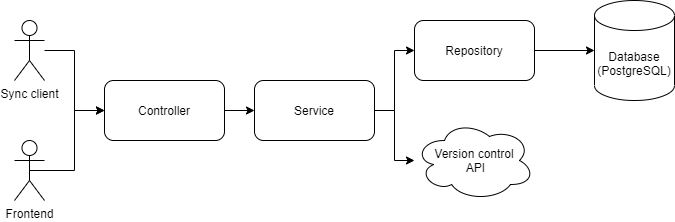
\includegraphics[width=\textwidth]{figures/backend_layered_diagram}
    \caption{Backend architecture}
    \label{fig:backend-layered-diagram}
\end{figure}

Folder structure is displayed in Table~\ref{tab:gtm-api-folder-structure}.
\begin{table}[h]
    \centering
    \begin{tabular}{ | p{3cm} | p{10cm} |}
        \hline
        \textbf{Folder} & \textbf{Purpose}\\
        \hline
        .github & CI/CD related files\\
        \hline
        migrations & Migrations for Diesel. \\
        \hline
        src/common & Widely used files.\\
        \hline
        src/db & General database connection.\\
        \hline
        src/domain & Main business logic.\\
        \hline
        src/security & Authentication and authorization.\\
        \hline
        src/vcs & Version control.\\
        \hline
        <root> & Configurations, README and LICENCE.\\
        \hline
    \end{tabular}
    \caption{Gtm-api folder structure.}
    \label{tab:gtm-api-folder-structure}
\end{table}

\subsection{Database design}\label{subsec:database-design}
One requirement for choosing the database, was that we needed it to have bindings for our Object-relational mapper (ORM),
so we could easily use it in our application.
This requirement narrowed the search down to SQLite, MySQL and PostgreSQL as they were the only languages with full support in Diesel.
There are other ORM-s written for Rust, but Diesel is one of the most popular ones, so we decided to go with it as
there was no need to use some other database.
% TODO: S6nastus paremaks

SQLite was ruled out as it is not strongly typed, and does not have the same amount of features PostgreSQL and MySQL have.
For deciding between MySQL and PostgreSQL it came down to personal preference as both of them are strongly typed and
support all the required features, including recursive queries.
Both of them are also open source.

We decided to go with PostgreSQL, as we had prior experience with it.

As we are running the application in "beta", we decided to run the database in a docker container on our development machine to
reduce the cost of upkeep.
For data persistence, we have mounted database files volume to the host machine.

\subsubsection{Database versioning}\label{subsubsec:database-versioning}
As we have users data in our database, it is important to also persist it through database schema updates.
For this, we use migrations and let Diesel handle the updates.
Every time database change is required, we add a new migration with both up and down scripts that can be used by Diesel
to run the migration or revert it.
Diesel is configured to automatically run updates added to the release.
As reverting database changes can result in a loss of data, it has to be done manually via Diesel CLI app.

\subsubsection{ERD Schema}\label{subsubsec:erd-schema}
The database holds data about tracked time, registered users and how the users can access time data.
The structure of the database schema is described in Figures~\ref{fig:erd-schema-user} and~\ref{fig:erd-schema-general}.

Time data follows the structure of the Git commits tree and file tree.
The \textit{repositories} table contains general information about the Git repository such as name and the sync client
responsible for tracking it.
The \textit{commits} table has the information about commits such as author, timestamp and commit message.
Each \textit{commits} table entry also has a reference to the repository it is committed to.
Every commit has zero or more files that were edited in it.
These files are contained in \textit{files} table, and they contain information about files added and deleted.
To have more accurate data about when the time was spent, separate table is needed as there is no guarantee that
the time spent editing files is spent just before the commit timestamp.
For this, we have a table called \textit{timeline}, which holds timestamps and durations of every consecutive edit as
well as a reference to a file in which the time was spent.

The \textit{users} and \textit{roles} tables are responsible for persisting user login credentials, roles and connected OAuth accounts.
As we allow the user to optionally register only via OAuth, the password field is nullable.
Users that have no password, can only log in via OAuth, but they can also add a password at any time.

Every user can have multiple rows with role \textit{USER} being added to every user by default.
There are three roles in total: \textit{USER}, \textit{LECTURER} and \textit{ADMIN}.
Currently, there are no rules in the database for any of the roles, which means all checks are done in software.
More detailed description about roles can be found in~\nameref{subsec:roles} subsection.

Every user also has zero or more OAuth logins stored in the \textit{logins} table.
There is a limit that every user can have at maximum one OAuth login per login type.
If one already exists, it is updated instead of adding a new.

User emails retrieved from OAuth providers are stored in the \textit{emails} table to avoid unnecessary web requests.

\begin{figure}[H]
    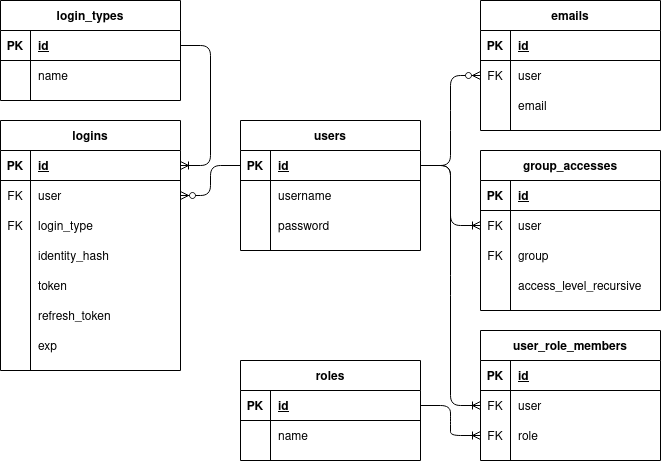
\includegraphics[width=\textwidth]{figures/erd_schema_user}
    \caption{ERD schema for user related tables}
    \label{fig:erd-schema-user}
\end{figure}

\begin{figure}[H]
    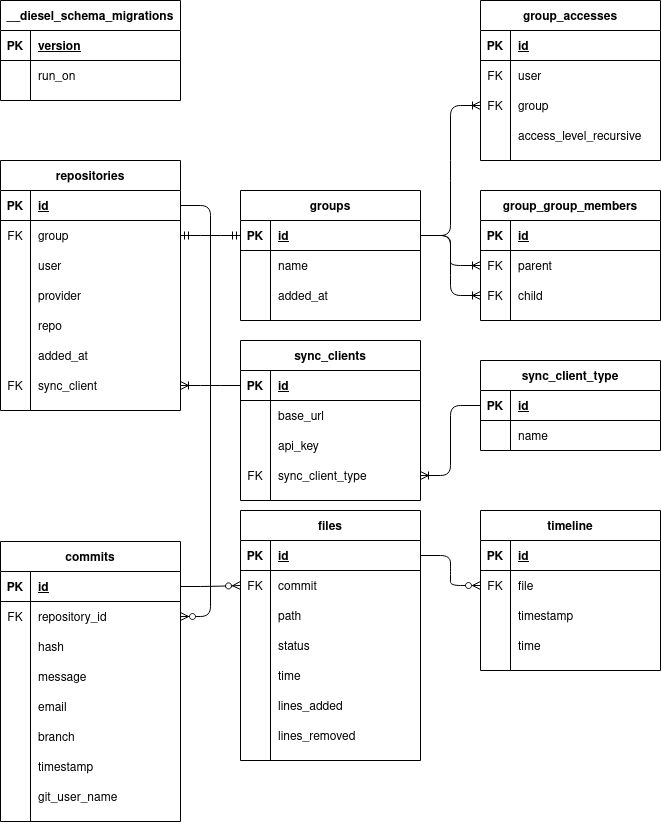
\includegraphics[width=\textwidth]{figures/erd_schema_general}
    \caption{ERD schema for non-user related tables}
    \label{fig:erd-schema-general}
\end{figure}

\section{Frontend}\label{sec:frontend}
A frontend is a software program or website that the user interacts with.
In our case, frontend is a website where the user can see time tracking data according to their privileges. %TODO his/her or their?
Although technically also CLI app can be considered frontend, when we refer to frontend we only mean the website.

The frontend has been built using ReactJS library.
According to the State of Frontend 2020 report, ReactJS is the most used JavaScript framework and also the framework, which developers want to learn or keep using the most.
It is faster than Angular, and its somewhat functional style was more appealing for us than the style of Vue.
It was chosen by Marten, who is mostly responsible for frontend development and has had some prior experience with it.
The most popular frontend frameworks are shown in Figure~\ref{fig:frontend-framework-popularity} sorted from most favored to less.

\begin{figure}[h]
    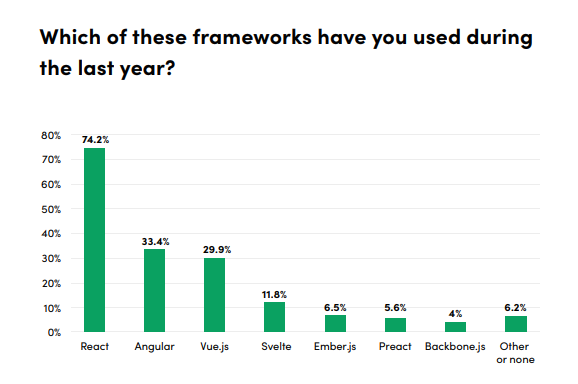
\includegraphics[width=\textwidth]{figures/frontend_framework_popularity}
    \caption{Frontend framework popularity~\cite{state-of-frontend-report}}
    \label{fig:frontend-framework-popularity}
\end{figure}

\subsection{Code design}\label{subsec:code-design}
Frontend code is written following the main principles promoted by ReactJS community and documentation.
For an example, component's names use \textit{PascalCase}, helper files use \textit{camelCase}, folders use \textit{camelCase}.
Code is divided into multiple files/components to prevent code repetition, inline CSS is avoided, the liner is used to make code easier to use, service calls are in the separate file, etc.
To improve code quality and readability TypeScript was chosen, as it is a strongly typed language, which JavaScript is not.
This decision was not made at the beginning of the project but as the code kept growing and readability suffered the decision was made.
One of the biggest reason for the switch from JavaScript to TypeScript was that due to being a strongly typed language,
TypeScript has better IDE support.
Folder structure is displayed in Table
\ref{tab:gtm-front-folder-structure}.

\begin{table}[h]
    \centering
    \begin{tabular}{ | p{3cm} | p{10cm} |}
        \hline
        \textbf{Folder} & \textbf{Purpose}\\
        \hline
        .github & CI/CD related files\\
        \hline
        src/api & Service calls .\\
        \hline
        src/assets & Images and icons. \\
        \hline
        src/containers & Main container structure (Header, Footer, Content, etc.)\\
        \hline
        src/models & Easy-Peasy state management models.\\
        \hline
        src/reusable & components that can be reused.\\
        \hline
        src/routes & Routes.\\
        \hline
        src/scss & Style.\\
        \hline
        src/store & Store for state management.\\
        \hline
        src/utils & Helpers.\\
        \hline
        src/views & Views that are used once.\\
        \hline
        <root> & TypeScript configuration, package.json, README and LICENCE.\\
        \hline
    \end{tabular}
    \caption{Gtm-front folder structure.}
    \label{tab:gtm-front-folder-structure}
\end{table}

\subsection{User interface design}\label{subsec:user-interface-design}
User interface must be built keeping the user in mind.
User experience is the most important part of a web application.
If the user does not have a good experience with the interface, it might be the end of the interaction between the user and the application.
Since the team did not have any professional designers, CoreUI was a great choice to make the design process much easier.
CoreUI is an Open Source Bootstrap Admin Template which is built on Bootstrap and written with readability in mind.
The design and easy usability were the decisive factors in choosing CoreUI.

However, CoreUI's charts were not customizable to the extent we required.
For better customization, Recharts was chosen for building graphics.
Recharts is a composable charting library built on React components and D3.
It is much more customizable than CoreUI charts as it allows combining different bar charts, line charts, etc.
\cite{recharts-readme}

At this point, the design problem arose again.
Designing graphs were done in the following manner:
\begin{enumerate}
    \item Understand the functionality and create an initial component.
    \item Let it settle for some time and then discuss with the team.
    \item Finalize component and release it for test users.
    \item Make final changes according to the users' feedback.
\end{enumerate}
Design patterns such as graph sizes, colours, spacings, fonts etc. were chosen in such a way that they would look similar to CoreUI graphs.

\subsection{State management}\label{subsec:state-management}
State management does not have a certain winner.
Choosing a state management library comes down to personal preference.
We decided to use Easy-Peasy, which is built on the most popular state management library Redux.
Easy Peasy was chosen over Redux because Redux has a steep learning curve but Easy-Peasy is easy to use.
%TODO: Vb contents alla?
